\subsubsection{Distributions of Features}\label{sssec:featdist}

\noindent The distribution for each feature in different forecasting periods was plotted using a third party library called \textbf{seaborn} \cite{python:seaborn}. The 4 moments (mean, standard deviation, skew and kurtosis) were also computed and shown in the plot. This was done to check whether a feature follows a normal distribution or not as shown in Figure \ref{fig:feature_dist}. The skew and kurtosis were computed using a third party library called \textbf{scipy.stats} \cite{python:scipy}. The plots show that the features are not normally distributed (both visually and the kurtosis being far off from 3), meaning that the features are in fact not normally distributed or there are extreme outliers (heavy tails). The plots also indicate that some features are highly skewed. 
\begin{figure}[H]
\centering
  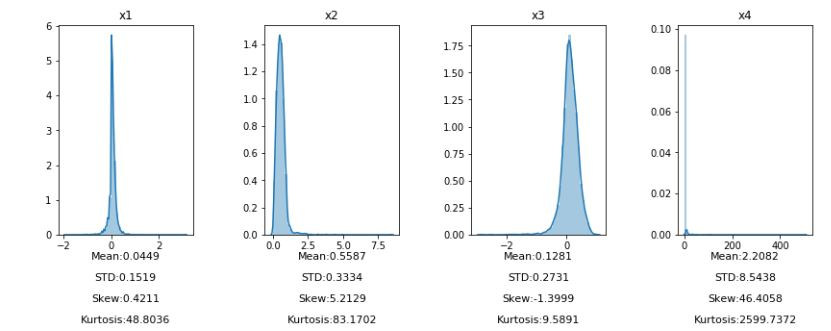
\includegraphics[scale = .7]{imgs/feature_distributions.JPG}
  \caption{A snippet for the distributions for each feature for Year 2 using \textbf{seaborn} and \textbf{scipy.stats}}
  \label{fig:feature_dist}
\end{figure}

